\section{Các khái niệm về xác suất}
\subsection{Hàm mật độ xác suất (Probability density function)}
Với các khối nến có các thành phần như giá mở, giá đóng, số lượng đồng giao dịch,..., ta có thể coi như các biến ngẫu nhiên liên tục tương ứng. Khái niệm hàm mật độ xác suất trong văn cảnh trên được hiểu như một hàm gồm các tham số thể hiện được mật độ phân bố của các biến ngẫu nhiên.
\begin{figure}[hbt!]
	\centering
	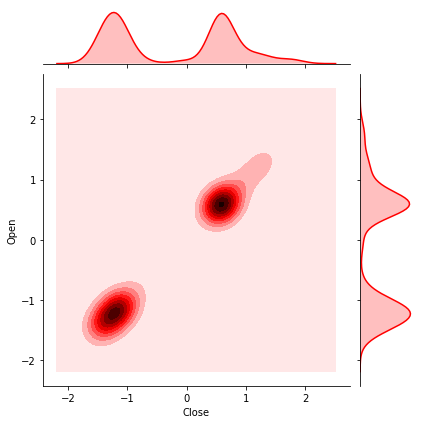
\includegraphics[width=0.8\textwidth]{probability/z_score_marginal_distribute_diff.png}
	\caption{Phân phối biên giá mở/đóng dữ liệu đã xử lý}
	\label{fig:z_score_marginal_distribution_diff}
\end{figure}
\FloatBarrier
Hình ~\ref{fig:z_score_marginal_distribution_diff} thể hiện mật độ của phân phối đồng thời giữa giá đóng và giá mở của các khối nến được biểu diễn dưới dạng $p_{data}(Open, Close)$.
\subsection{Hàm phân phối biên (Marginal distribution)}
Với dữ liệu liên tục như trên, hàm phân phối biên đối với giá mở được biểu diễn dưới dạng:
$p_{data}(Open) = \int_y p_{data}(Open, Close=y) dy = \int_y p_{data}(Open \given Close=y)p_{data}(Close=y)dy$ Một cách trực quan, hàm phân phối trên được biểu diễn bởi đường biên bên trái Hình ~\ref{fig:z_score_marginal_distribution_diff}

\subsection{Nhiễu dữ liệu}
Nhiễu trong dữ liệu như phần đề cập trong chương